
Le lissage spline donne une fonction de classe $\mathcal C^2$, ce qui est un désavantage dans le cadre du prélissage qui sert à déterminer les paramètres de régularité de courbes issues d'un processus que l'on ne suppose pas plus régulier que continu. Toutefois, le fait d'utiliser une base de fonctions pour effectuer le lissage a de nombreux avantages par rapport au lissage à noyaux qui peuvent éventuellement s'avérer utiles dans certaines situations spécifiques pour la mise en production de modèles.

En effet, une fois que l'on a déterminé les composantes de la décomposition de notre signal sur la base de fonctions, on n'a plus besoin de se référer aux données pour prédire une valeur. Il s'agit d'une méthode très économe en mémoire, ce qui peut être très avantageux dans le cadre de la mise en production de modèles lorsqu'il y a de nombreuses courbes observées.

\section{Ondelettes}
\subsection{Une brève introduction aux ondelettes}


Les ondelettes proviennent du monde du traîtement du signal. Elles répondent à un problème de représentation des données à la fois dans le domaine temporel et dans le domaine fréquentiel. En effet, la transformée de Fourier nous donne accès aux fréquences présentes dans un signal mais ne nous permet pas de localiser à quel moment sont intervenues les fréquences spécifiques. Le théorème d'indétermination de Heisenberg stipule que l'on ne peut avoir une résolution parfaite à la fois dans le domaine fréquentiel et le domaine temporel, il y a un compromis qui doit être fait. La question devient alors :

\question{
	\smallskip\centering
	Comment représenter une fonction dans le domaine temporel et dans le domaine fréquentiel de façon optimale ? En d'autres termes, quelle résolution temporelle et quelle résolution fréquentielle choisir ?
}

Une première approche proposée en 1946 par Denis Gabor est la transformée de Fourier à court terme (STFT). Celle-ci consiste à regarder la transformée de Fourier d'une fonction sur une fenêtre de taille fixe et à faire glisser cette fenêtre sur la fonction. On obtient ainsi la représentation fréquentielle de la fonction sur un intervalle de temps centré en un point que l'on peut faire varier.

\bigskip

\begin{minipage}{0.32 \textwidth}
	\begin{figure}[H]
		\centering
		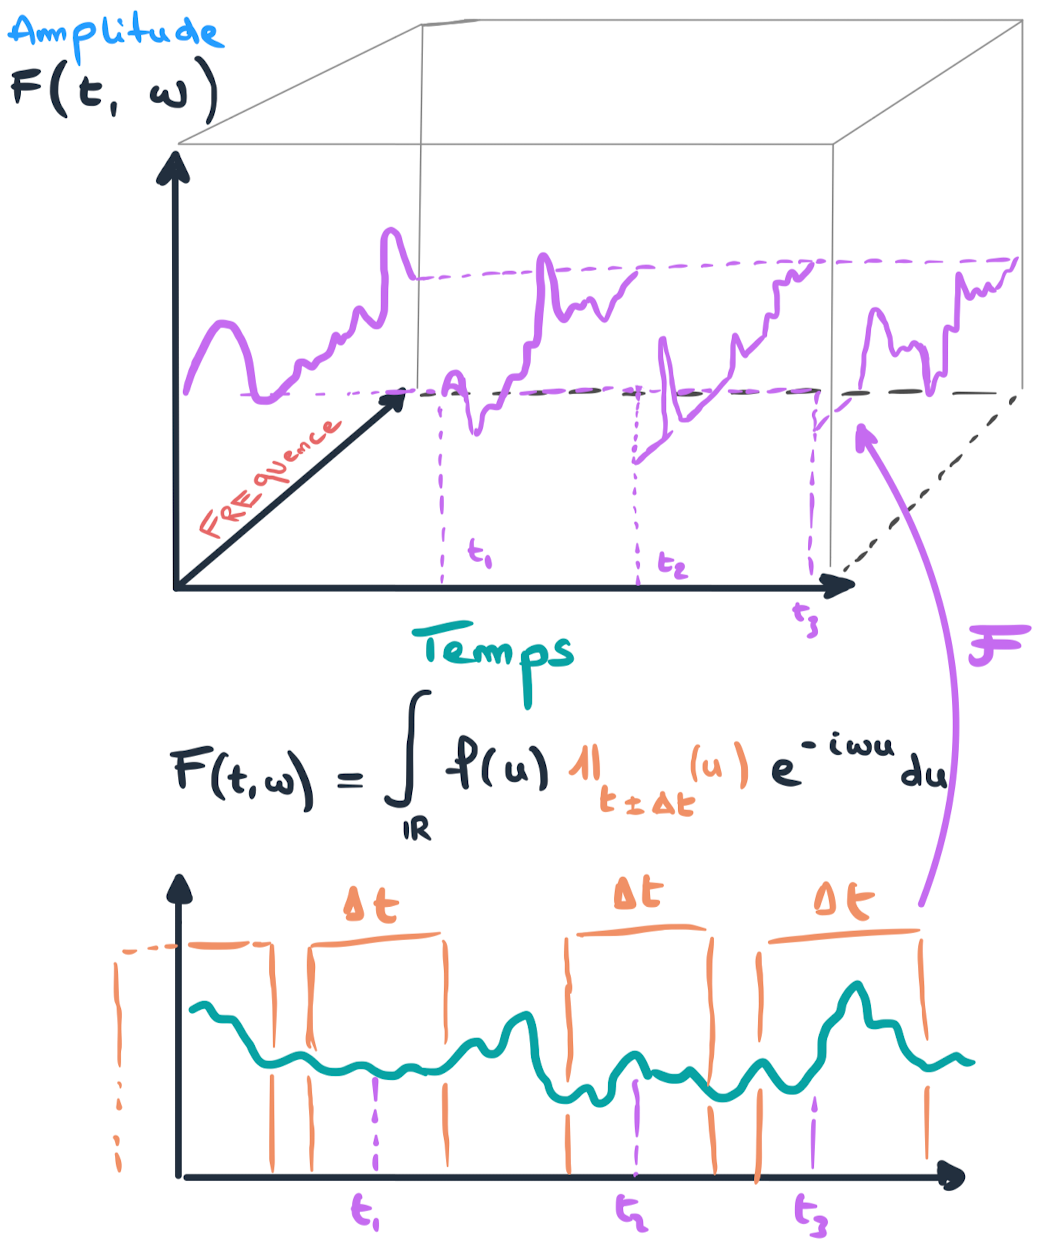
\includegraphics[width=\textwidth]{images/sketches/STFT.png}
		\caption{Transformée de Fourier à court terme d'une fonction}
		\label{fig:STFT}
	\end{figure}
\end{minipage}
\hfill
\begin{minipage}{0.60 \textwidth}

	Cependant contrairement à ce que peut suggérer le dessin présenté ici, la résolution fréquentielle n'est pas parfaite. Elle est d'ailleurs dans le cadre de la Transformée de Fourier à court terme constante, que ce soit sur le domaine temporel ou le domaine fréquentiel. La résolution fréquentielle est donc constante quelque soit la fréquence considérée.

	\question{
		\smallskip\centering
		Quel est le problème avec cette approche ?
	}

	le problème ne vient pas du monde mathématique mais plutôt du monde réel : les signaux que l'on observent présentent la caractéristique suivante : Les signaux de basse fréquence ont tendance à s'étendre sur la durée, et les signaux de hautes fréquences ont tendance à être très localisées, sous forme d'impulsion. Il devient alors clair que pour correctement identifier et localiser les fréquences présentes dans un signal, il est judicieux (voire parfois nécessaire) de varier la résolution fréquentielle et temporaire (limitées par le théorème d'indétermination de Heisenberg) en fonction de ce qui est le plus difficile à distinguer. C'est ce que proposent les ondelettes.

\end{minipage}


\subsection{Motivation dans le cadre de l'analyse de données fonctionnelles}

La capacité de capturer de façon efficiente les irrégularités\footnote{on pourra se référer pour la justification technique de cette affirmation l'annexe \ref{annexe:wavelet}} de la fonction lissée est une motivation pour l'utilisation de la base d'ondelettes pour effectuer le pré-lissage de données, dont on espère qu'il n'écrase pas la majorité de l'information irrégulière de nos données. Si une des méthodes possibles, comme mentionnée précédemment, est d'utiliser un lissage non paramétrique à noyaux, les bases de fonctions ont de nombreux avantages. Un des avantage est le fait qu'une fois les projections sur la base déterminées, il n'y a plus besoin de se référer de nouveau aux données originales par la suite. Cela donne une représentation très parcimonieuse des données. Alors pour déterminer la valeur de $\widehat X(t)$ en un point $t$ non observé, il suffit d'évaluer l'expression $\sum_k \prodscal X {\psi_k} \psi_k(t)$ avec $(\psi_k)_{k \in \llbracket 1, K \rrbracket}$ la base d'ondelettes tronquée déterminée par validation croisée.
